\documentclass[a4page]{article}
\usepackage[T1]{fontenc}
\usepackage[utf8]{inputenc}
\usepackage[italian]{babel}
\usepackage{index}
\usepackage{booktabs}
\usepackage{longtable}
\usepackage{array}
\usepackage{graphicx}
\usepackage{ulem}
\usepackage[table,xcdraw]{xcolor}
\usepackage[T1]{fontenc}
\usepackage{xcolor,listings}
\usepackage[vmargin=2cm]{geometry}
\usepackage{color}
\usepackage{lscape}
\usepackage{imakeidx}
\usepackage{fancyvrb}

\usepackage{titlesec, blindtext, color}
\definecolor{gray75}{gray}{0.75}
\usepackage{textcomp}
    \usepackage{color}

    \definecolor{codegreen}{rgb}{0,0.6,0}
    \definecolor{codegray}{rgb}{0.5,0.5,0.5}
    \definecolor{codepurple}{HTML}{C42043}
    \definecolor{backcolour}{HTML}{F2F2F2}
    \definecolor{bookColor}{cmyk}{0,0,0,0.90}  
    \color{bookColor}

    \lstset{upquote=true}

    \lstdefinestyle{mystyle}{
        backgroundcolor=\color{backcolour},   
        commentstyle=\color{codegreen},
        keywordstyle=\color{codepurple},
        numberstyle=\footnotesize\color{codegray},
        stringstyle=\color{codepurple},
        basicstyle=\footnotesize,
        breakatwhitespace=false,         
        breaklines=true,                 
        captionpos=b,                    
        keepspaces=true,                 
        numbers=left,                    
        numbersep=-10pt,                  
        showspaces=false,                
        showstringspaces=false,
        showtabs=false,      
    }
    \lstset{style=mystyle} 
\newcommand{\hsp}{\hspace{20pt}}
\titleformat{\chapter}[hang]{\Huge\bfseries}{\thechapter\hsp\textcolor{gray75}{|}\hsp}{0pt}{\Huge\bfseries}

\begin{document}
% inizio pagina@@@@
\clearpage
% command to provide stretchy vertical space in proportion
\newcommand\nbvspace[1][3]{\vspace*{\stretch{#1}}}
% allow some slack to avoid under/overfull boxes
\newcommand\nbstretchyspace{\spaceskip0.5em plus 0.25em minus 0.25em}
\begin{titlepage}
\begin{center}
\tt
\nbvspace[0.03]
\begin{tabular}[c]{@{}c@{}}\vspace{0.1cm}\textbf{\LARGE{UNIVERSITA' DEGLI STUDI DI NAPOLI FEDERICO II}}\\\vspace{0.1cm}\Large{SCUOLA POLITECNICA E DELLE SCIENZE DI BASE}\\\large{DIPARTIMENTO DI INGEGNERIA ELETTRICA E TECNOLOGIE DELL'INFORMAZIONE}\end{tabular}

\includegraphics[width=4cm]{LOGO}
\nbvspace[0.1]
\begin{tabular}[c]{@{}c@{}}\vspace{0.1cm}\Large{CORSO DI LAUREA IN INFORMATICA}\\\vspace{0.1cm}\Large{INSEGNAMENTI DI BASI DI DATI E PROGRAMMAZIONE AD OGGETTI}\\\Large{ANNO ACCADEMICO 2022/2023}\end{tabular}
\rm
\begin{tabular}[c]{@{}c@{}}\huge{\textbf{Progettazione e sviluppo di una base di dati}}\\\huge{\textbf{relazionale per la descrizione e la}}\\\huge{\textbf{memorizzazione di conferenze scientifiche}}\end{tabular}
\end{center}
\begin{longtable}[c]{llr}
\textit{Autori:}                                                                                                                   &  & \textit{Docenti:}                                                                        \\
\endhead
%
\begin{tabular}[c]{@{}l@{}}ALESSANDRO GRIECO\\      Matricola N86/4241\\      alessandro.grieco2@studenti.unina.it\end{tabular}    &  & \begin{tabular}[c]{@{}r@{}}Prof. Mara SANGIOVANNI\end{tabular} \\
\begin{tabular}[c]{@{}l@{}}GIANFRANCO DUMINUCO\\      Matricola N86/4061\\      gianfranco.duminuco@studenti.unina.it\end{tabular} &  & \multicolumn{1}{l}{}                                                                    
\end{longtable}                  
\end{titlepage}
\tableofcontents
\newpage
\section{PREFAZIONE}
Si provvederà alla progettazione e sviluppo di una base di dati dedicata alla gestione di conferenze. La base di dati permetterà di effettuare modifiche a conferenze già esistenti, di inserire conferenze future e visualizzare specifici dati riguardanti tutto ciò di cui una conferenza è composta.
\subsection{Conferenza, sede, programma, locazione e sessione}
Questo insieme di entità sono lo scheletro di una conferenza, permettono di identificare le informazioni sulla data/orario/luogo della conferenza:
\begin{itemize}
\item \textbf{conferenza} : Fornisce dati generali sulla trattazione e organizzazione temporale della conferenza;
\item \textbf{programma e sessione} : Consentono di conoscere gli orari e argomenti delle varie sedute della conferenza;
\item \textbf{sede e locazione} : Definiscono il luogo fisico in cui si terranno le varie sessioni di una conferenza.
\end{itemize}
\subsection{Evento sociale e intervallo}
Consentono ad un partecipante e/o ad un organizzatore di identificare i momenti di pausa ed i momenti di eccezione di una conferenza
\subsection{Organizzatore locale, organizzatore scientifico, partecipante, intervento ed ente}
Questo gruppo di entità costituisce la base delle varie sessioni di una conferenza. Compongono la popolazione di una conferenza, come questa partecipa alle varie sessioni e come questa si muove all'interno di una conferenza.
\begin{itemize}
\item \textbf{ente} : Specifica l'ente di appartenenza di ciascun elemento appartenente alla popolazione di una conferenza;
\item \textbf{Organizzatore locale e scientifico} : Definisce le persone fisiche che organizzano una conferenza;
\item \textbf{partecipante e intervento} : Il partecipante è lo spettatore fisico di una sessione, il quale può intervenire o meno all'interno di essa.
\end{itemize}
\subsection{Sponsor e pubblicità}
Determinano l'insieme delle aziende le quali contribuiscono (anche economicamente) alla realizzazione di una conferenza.
\newpage
\section{PROGETTAZIONE CONCETTUALE}
In seguito sono riportati il diagramma ER e il rispettivo class diagram:
\subsection{ER}
\begin{figure}[h!]
\centering
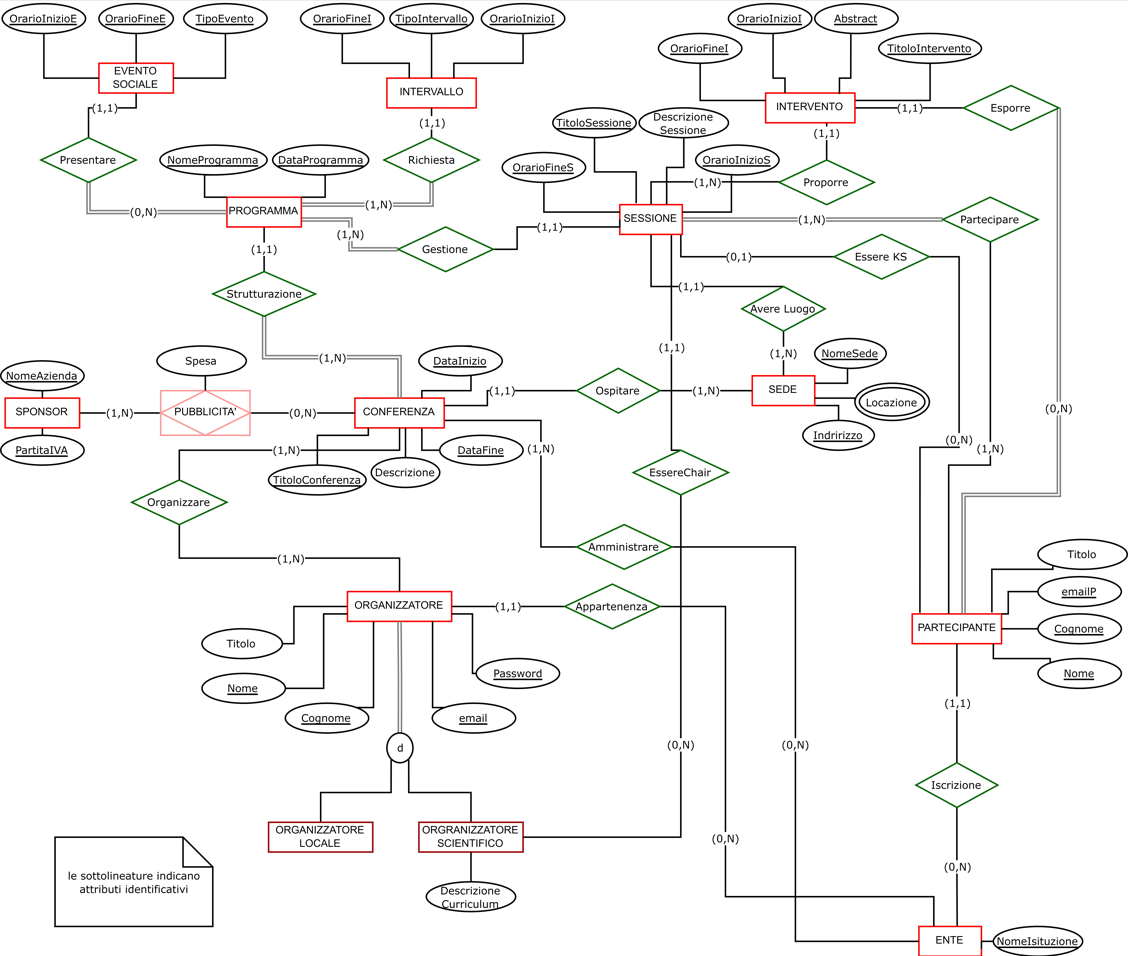
\includegraphics[]{ER}
\end{figure}
\newpage
\subsection{CLASS DIAGRAM}
\begin{figure}[h!]
\centering
\includegraphics[width=17cm]{CSNR}
\label{mycsnr}
\end{figure}
\newpage
\subsection{Ristruttuazione del class diagram}
Per motivi di implementazione fisica è necessario ristrutturare il class diagram sopracitato \ref{mycsnr}, tenendo conto dei seguenti punti.
\subsection{Eliminazione attributi multivalore}
L'unico attributo multivalore presente nel diagramma risulta essere l'attributo locazione nell'entità sede, quindi è necessario rendere quest'ultimo un entità a sé stante. 
% aggiungere foto dettagliata su locazione e come diventa%
\subsection{Eliminazione attributi strutturati}
L'unico attributo strutturato risulta essere l'attributo indirizzo all'interno dell'entità sede, il quale può essere ristrutturato componendolo nei suoi sotto-attributi (NomeVia, NumeroCivico, Città)
% aggiungere foto dettagliata su indirizzo e come diventa%
\subsection{Scelta degli identificatori primari}
Per le entità sessione, programma, conferenza, intervento, intervallo, evento sociale sono state introdotte delle chiavi surrogate (rispettivamente codsessione, codprogramma, codconferenza, codintervento, codintervallo, codevento). \vspace{1cm}\newline
Per le entità sponsor, partecipante, organizzatore locale, organizzatore scientifico, ente, locazione e sede sono stati identificate come chiavi attributi preesistenti (rispettivamente PartitaIva, emailP, emailL, emailS, NomeIstituzione, NomeLocazione, NomeSede).
\subsection{Eliminazioni delle gerarchie}
L'unica gerarchia identificata (totale e disgiunta) nel class diagram è quella tra organizzatore, organizzatore scientifico ed organizzatore locale. Poiché l'entità organizzatore scientifico è composta da un attributo non presente in organizzatore locale ed è connesso a sessione tramite la relazione \textit{EssereChair} è possibile andare ad accorpare gli attributi dell'entità padre all'interno delle entità figlie.
% aggiungere foto bla bla%
\subsection{Analisi delle ridondanze}
Nel class diagram non sono presenti ridondanze.
\newpage
\subsection{CLASS DIAGRAM RISTRUTTURATO}
\begin{figure}[h!]
\includegraphics[width=18cm]{CSR}
\end{figure}


\subsection{Dizionario classi}

\setlength{\LTleft}{-70pt}
\setlength\LTright{0pt}
\renewcommand\arraystretch{1.5}
\begin{longtable}{@{\extracolsep{\fill}}ccl}
\toprule
\multicolumn{1}{c}{\textbf{CLASSE}} & \multicolumn{1}{c}{\textbf{DESCRIZIONE}}                                                                                                                                                     & \textbf{ATTRIBUTI}                                                                                                                                                                                                                                                                                                                                                                                                                                                                                                                                                                                                                                                                                                                          \\ \bottomrule
\endhead
%
\textbf{CONFERENZA}                 & \begin{tabular}[c]{@{}c@{}}\vspace{-0.2cm}Riunione di rappresentanti di vari enti, \\ \vspace{-0.2cm}per uno scambio di vedute su problemi \\ \vspace{-0.2cm}di attualità o per risolvere una controversia \\ internazionale\end{tabular} & \begin{tabular}[c]{@{}l@{}}\vspace{-0.2cm}\textbf{CodConferenza} (integer): Chiave tecninca.\\ \vspace{-0.2cm}Identifica univocamente ciascuna istanza\\ di Conferenza.\\\vspace{-0.2cm}\textbf{DataInizio} (date) : Data che ha luogo la \\ Conferenza.\\ \vspace{-0.2cm}\textbf{DataFine} (data) : Data ove termina \\la Conferenza.\\ \vspace{-0.2cm}\textbf{Descrizione} (string) : Testo che illustra \\gli obiettivi della Conferenza.\\\vspace{-0.2cm}\textbf{TitoloConferenza} (string) : Nome che identifica \\la Conferenza.\end{tabular}                                                                                     \\ \hline
\textbf{SEDE} & \begin{tabular}[c]{@{}c@{}}Luogo fisico ove si tiene la conferenza\end{tabular} &\begin{tabular}[c]{@{}l@{}}\vspace{-0.2cm}\textbf{NomeSede} (string) : Nome identificativo \\\vspace{-0.2cm}della sede. Identifica univocamente le istanze\\ di Sede.\\\vspace{-0.2cm}\textbf{NomeVia} (string) : Nome nella strada in \\cui è presente la Sede.\\\vspace{-0.2cm}\textbf{NumeroCivico} (integer):Numero effettivo\\ della strada\\\vspace{-.2cm}\textbf{Città} (string): Comune dove è presente\\la Sede\end{tabular}
\\ \hline
\textbf{LOCAZIONE} & \begin{tabular}{@{}c@{}}\vspace{-0.2cm}Struttura interna alla sede \\ove si tiene la sessione \end{tabular} & \begin{tabular}{@{}l@{}}\vspace{-0.2cm}\textbf{NomeLocazione} (string) : Nome della\\locazione

\end{tabular} \\ \hline
\textbf{PROGRAMMA}                  & \begin{tabular}[c]{@{}c@{}}\vspace{-.2cm}Gestore della conferenza per migliorare\\ \vspace{-.2cm}la programmazione degli eventi\\ della conferenza\end{tabular}                                                          & \begin{tabular}[c]{@{}l@{}}\vspace{-.2cm}\textbf{CodProgramma} (integer) : Chiave tecnica.\\ \vspace{-.2cm} Identifica univocamente ciascuna istanza\\ di Programma.\\\textbf{DataProgramma} (date) : Data del programma\end{tabular}                                                                                                                                                                                                                                                                                                                                                                                                                                                                                                                                                                                                                                                                   \\ \hline
\textbf{SESSIONE}                   & \begin{tabular}[c]{@{}c@{}}\vspace{-.2cm}Frammento di una conferenza avvenuta\\ in una data in un certo orario\end{tabular}                                                                                & \begin{tabular}[c]{@{}l@{}}\vspace{-.2cm}\textbf{CodSessione} (integer) : Chiave tecnica.\\\vspace{-.2cm} Identifica univocamente le istanze\\ di Sessione.\\\vspace{-.2cm}\textbf{OrarioInizioSessione} (time) : Orario inizio\\ della Sessione \\\vspace{-.2cm}\textbf{OrarioFineSessione} (time) : Orario fine della\\ Sessione.\\\vspace{-.2cm}\textbf{TitoloSessione} (string) : Denominazione\\ identificatrice della Sessione\\\vspace{-.2cm}\textbf{DescrizioneSessione} (string) : Testo illustrativo\\ degli obiettivi e discussione della Sessione.\\\vspace{-.2cm}\textbf{Chair} (string) : Organizzatore scintificato che\\ coordina la Sessione identificato con l'email\\\vspace{-.2cm}\textbf{Keynote Speaker} (string) : Partecipante di \\\vspace{-.2cm}rilievo di una sessione, identificato\\ con l'email\end{tabular} \\ \hline
\textbf{PARTECIPANTE}               & \begin{tabular}[c]{@{}c@{}}\vspace{-0.2cm}Persona che partecipa\\ \vspace{-0.2cm}alla sessione in veste di\\ partecipante\end{tabular}                                                                                     & \begin{tabular}[c]{@{}l@{}}\vspace{-0.2cm}\textbf{emailP} (string): Indirizzo di posta elettrinica\\ \vspace{-0.2cm}del Partecipante. Identifica univocamente le\\ istanze di partecipante.\\ \vspace{-0.2cm}\textbf{Titolo} (TipoTitolo) : Carica accademica, professionale\\ o scientifica di rilievo (ex: dott./dott.ssa).\\ \textbf{Nome} (string) : Nome del partecipante.\\\textbf{Cognome} (string) : Cognome del partecipante.\\ \vspace{-0.2cm}\textbf{Istituzione\_di\_Afferenza} (string) : Nome dell'\\ Istituto che afferisce il Partecipante.\end{tabular}                                                                                                                                                                                                                                                                                                                                                  \\ \hline
\textbf{INTERVENTO}                 & \begin{tabular}[c]{@{}c@{}}\vspace{-0.2cm}L'atto di prendere la parola\\  \vspace{-0.2cm}al fine di metter luce su\\ argomenti inerenti alla sessione\end{tabular}                                                         & \begin{tabular}[c]{@{}l@{}}\vspace{-0.2cm}\textbf{CodIntervento} (string) : Chiave tecnica.\\\vspace{-0.2cm} Identifica univocamente le istanze\\ di Intervento.\\ \vspace{-0.2cm}\textbf{OrarioInizioIntervento} (time) : Orario\\ che ha inizio l'Intervento.\\ \vspace{-0.2cm}\textbf{OrarioFineIntervento} (time) : Orario che\\ termine l'Intervento.\\ \vspace{-0.2cm}\textbf{Abstract } (string) : Breve testo il cui contenuto\\ descrive cosa verrà presentato dall'Intervento.\end{tabular}                                                                                                                                                                                                                                                                                                                                                                                                                        \\ \hline
\textbf{PUBBLICITA'}                 & \begin{tabular}[c]{@{}c@{}}\vspace{-0.2cm}Identifica il costo a spese dell'azienda\\ nel farsi pubblicità nella conferenza. \end{tabular}                                                         & \begin{tabular}[c]{@{}l@{}}\vspace{-0.2cm}\textbf{Spesa} (Money) : Costo pubblicitario per l'azienda\end{tabular}                                                                                                                                                                                                                                                                                                                                                                                                                        \\ \hline
\textbf{EVENTO SOCIALE}             & \begin{tabular}[c]{@{}c@{}}\vspace{-0.2cm}Celebrazione o commemorazione di\\ \vspace{-0.2cm}un particolare momento trascorso\\\vspace{-0.2cm} tra persone interessate alla tematica\\ della conferenza\end{tabular}                       & \begin{tabular}[c]{@{}l@{}}\vspace{-0.2cm}\textbf{CodEvento} (integer) :  Chiave tecnica.\\ \vspace{-0.2cm}Identifica univocamente le istanze di\\ Evento Sociale.\\ \vspace{-0.2cm}\textbf{TipoEvento} (evento) : Enumerazione\\ che specifica il tipo di evento (ex: Cena).\\ \vspace{-0.2cm}\textbf{OrarioInizioEvento} (time) : Orario d'inizio\\ dell'evento sociale.\\\vspace{-0.2cm}\textbf{OrarioFineEvento} (time) : Orario fine dell'evento \\ sociale.\end{tabular}                                                                                                                                                                                                                                                                                                                                                                                                                                              \\ \hline
\textbf{INTERVALLO}                 & \begin{tabular}[c]{@{}c@{}}\vspace{-0.2cm}Breve interruzione di un programma\\ \vspace{-0.2cm}o sessione che consente ai\\\vspace{-0.2cm} partecipanti di riposarsi prima della\\ sua continuazione\end{tabular}                          & \begin{tabular}[c]{@{}l@{}}\vspace{-0.2cm}\textbf{CodIntervallo} (integer) : Chiave tecnica.\\ \vspace{-0.2cm}Identifica univocamente le istanze\\ di Intervallo.\\ \vspace{-0.2cm}\textbf{TipoIntervallo} (pausa) : Enumazione che\\ specifica il tipo di intervallo (ex: coffee break)\\ \vspace{-0.2cm}\textbf{OrarioInizioIntervallo} (time) : Orario d'inizio \\ dell'Intervallo.\\ \vspace{-0.2cm}\textbf{OrarioFineIntervallo} (time) : Orario di fine\\ Intervallo\end{tabular}                                                                                                                                                                                                                                                                                                                                                                                                                                     \\ \hline
\textbf{\begin{tabular}[c]{@{}c@{}}ORGANIZZATORE\\ SCIENTIFICO\end{tabular}} & \begin{tabular}[c]{@{}c@{}}\vspace{-0.2cm}Responsabile della gestione\\\vspace{-0.2cm} su tematiche scientifiche e \\\vspace{-0.2cm} saccente su uno dei campi \\ che afferiscono alla conferenza\end{tabular}                            & \begin{tabular}[c]{@{}l@{}}\vspace{-0.2cm}\textbf{emailS} (string) : Indirizzo di posta elettronica.\\ \vspace{-0.2cm}Identifica univocamente le istanze di Organizzatore\\ Scientifico.\\ \vspace{-0.2cm}\textbf{DescrizioneCurriculum} (string) : Presentazione\\ \vspace{-0.2cm}delle esperienze professionali e competenze\\ di un Organizzatore Scientifico.\\ \vspace{-0.2cm}\textbf{Titolo} (TipoTitolo) :Carica accademica o professionale\\ o personale di rilievo (ex: dott./dtt.ssa).\\ \vspace{-0.2cm}\textbf{Nome} (string): Nome dell'organizzatore\\ scientifico\\ \vspace{-0.2cm}\textbf{Cognome} (string) : Cognome dell'organizzatore\\ scientifico\\ \vspace{-0.2cm}\textbf{Istituzione\_di\_Afferenza} (string) : Nome dell'\\ istituto che afferisce l'organizzatore scientifico\end{tabular}                                                                                                                                                                              \\ \hline
\textbf{\begin{tabular}[c]{@{}c@{}}ORGANIZZATORE\\ LOCALE\end{tabular}}      & \begin{tabular}[c]{@{}c@{}}\vspace{-0.2cm}Responsabile della gestione tecnica\\ e logistica della conferenza\end{tabular}                                                                                     & \begin{tabular}[c]{@{}l@{}}\vspace{-0.2cm}\textbf{emailL} (string) : Indirizzo di posta elettronica.\\ \vspace{-0.2cm}Indentifica univocamente le istanze di organizzatore\\ locale.\\ \vspace{-0.2cm}\textbf{Titolo} (TipoTitolo) : Carica accademica, professionale o \\ personale di rilievo.\\ \vspace{-0.2cm}\textbf{Nome} (string) :Nome dell'organizzatore locale.\\ \vspace{-0.2cm}\textbf{Cognome} (string) : Cognome dell'organizzatore\\ locale.\\\vspace{-0.2cm}\textbf{Istituzione\_di\_Afferenza} (string) : Nome dell'istituto\\ che afferisce l'organizzatore locale.\end{tabular}                                                                                                                                                                                                                                                                                                                                                      \\ \hline
\textbf{ENTE}                       & \begin{tabular}[c]{@{}c@{}}\vspace{-0.2cm}Istituzioni che ideano la conferenza\\ definendone gli organizzatori\end{tabular}                                                                                 & \begin{tabular}[c]{@{}l@{}}\vspace{-0.2cm}\textbf{NomeIstituzione} (string) : Nome dell'istuto\\ che gestisce la conferenza.\end{tabular}                                                                                                                                                                                                                                                                                                                                                                                                                                                                                                                                                                                                                                                                                             \\ \hline
\textbf{SPONSOR}                    & \begin{tabular}[c]{@{}c@{}}\vspace{-0.2cm}Azienda interessata a promuoversi\\ \vspace{-0.2cm}pubblicizzandosi attraverso un\\ sostegno finanziario\end{tabular}                                                            & \begin{tabular}[c]{@{}l@{}}\vspace{-0.2cm}\textbf{PartitaIva} (string) : Codice identificativo di chi\\ svolge un'attività d'impresa o di lavoro autonomo.\\\textbf{NomeAzienda} (string) : Nome dell'azienda.\end{tabular}                                                                                                                                                                                                                                                                                                                                                                                                                                                                                                                  
		\\ \hline \bottomrule
\end{longtable}
\subsection{Dizionario associazioni}
\setlength{\LTleft}{-70pt}
\setlength\LTright{0pt}
\renewcommand\arraystretch{1.5}
\begin{longtable}{@{\extracolsep{\fill} }ccl}
\hline
\textbf{NOME}            & \textbf{DESCRIZIONE}                                                                                                                                   & \multicolumn{1}{c}{\textbf{CLASSI COINVOLTE}}                                                                                                                                                                                                                                                                                             \\ \hline
\endhead
%
\textbf{Strutturazione}  & \begin{tabular}[c]{@{}c@{}}\vspace{-0.2cm}Definisce la struttura di una conferenza \\ in base al programma assegnatogli.\end{tabular}                                 & \begin{tabular}[c]{@{}l@{}}
\textbf{Conferenza}{[}\textbf{1..*}{]}\vspace{-0.2cm} (\textit{è strutturata da}): specifica i \\ programmi di una Conferenza.\\ \textbf{Programma}{[}\textbf{1}{]}\vspace{-0.2cm}(struttura): specifica a quale\\ Conferenza è assegnato il nostro Programma.\end{tabular}                                                                                                                 \\ \hline
\textbf{Amministrare}    & \begin{tabular}[c]{@{}c@{}}\vspace{-0.2cm}Definisce la relazione tra le conferenze\\ e gli enti organizzatori delle stesse.\end{tabular}                              & \begin{tabular}[c]{@{}l@{}}\textbf{Conferenza}{[}\textbf{1..*}{]}\vspace{-0.2cm}(\textit{è amministrata da}): specifica \\\vspace{-0.2cm} quali enti contribuiscono nell'organizzazione \\della conferenza. \\ \vspace{-0.2cm}\textbf{Ente}{[}\textbf{0..*}{]}(\textit{amministra}): specifica quali \\ conferenze sono amministrate da un ente.\end{tabular}                                                                               \\ \hline
\textbf{Essere Chair}    & \begin{tabular}[c]{@{}c@{}}\vspace{-0.2cm}Definisce il ruolo "essere chair" da parte\\\vspace{-0.2cm} di un organizzatore scientifico in \\ realzione con una sessione.\end{tabular} & \begin{tabular}[c]{@{}l@{}}\vspace{-0.2cm}\textbf{Sessione}{[}\textbf{1}{]}(\textit{ha come chair}): specifica chi è il\\ chair di una determinata sessione.\\\vspace{-0.2cm}\textbf{Organizzatore\_Scientifico}{[}\textbf{0..*}{]}(\textit{è chair di}): \\\vspace{-0.2cm} specifica di quali sessioni un organizzatore è\\ chair.\end{tabular}                                                                                           \\ \hline
\textbf{Pubblicizza}     & \begin{tabular}[c]{@{}c@{}} \vspace{-0.2cm}Definisce la relazione di \\\vspace{-0.2cm} sponsorizzazione tra le conferenze\\ e i suoi sponsor.\end{tabular}                            & \begin{tabular}[c]{@{}l@{}}\vspace{-0.2cm}\textbf{Sponsor}{[}\textbf{1..*}{]}(\textit{pubblicizza}):specifica quali \\ conferenze sono pubblicizzate da uno sponsor.\\ \vspace{-0.2cm}\textbf{Conferenza}{[}\textbf{0..*}{]}(\textit{è pubblicizzata da}): specifica\\ da quale sponsor una conferenza è pubblicizzata.\end{tabular}                                                                                          \\ \hline
\textbf{Organizzare\_L}  & \begin{tabular}[c]{@{}c@{}}\vspace{-0.2cm}Definisce la relazione tra le conferenze \\\vspace{-0.2cm} e gli organizzatori locali che\\ le organizzano.\end{tabular}                   & \begin{tabular}[c]{@{}l@{}}\vspace{-0.2cm}\textbf{Organizzatore\_Locale{[}1..*{]}}(\textit{è organizzatore locale di}):\\ \vspace{-0.2cm}specifica quali sono le conferenze che un \\ organizzatore locale gestisce. \\ \vspace{-0.2cm}\textbf{Conferenza{[}1..*{]}}(\textit{ha come organizzatore locale}):\\ \vspace{-0.2cm}specifica chi sono gli organizzatori locali che\\ gestiscono la conferenza.\end{tabular}                    \\ \hline
\textbf{Organizzare\_S}  & \begin{tabular}[c]{@{}c@{}}\vspace{-0.2cm}Definisce la relazione tra le \\ \vspace{-0.2cm}conferenze e gli organizzatori scientifici \\ che la organizzano.\end{tabular}             & \begin{tabular}[c]{@{}l@{}}\vspace{-0.2cm}\textbf{Organizzatore\_Scientifico{[}1..*{]}}\\ \vspace{-0.2cm}(\textit{è organizzatore scientifico di}): specifica quali sono\\ le conferenze che un organizzatore locale gestisce.\\\vspace{-0.2cm} \textbf{Confernza{[}1..*{]}}(\textit{ha come organizzatore scientifico}):\\ \vspace{-0.2cm} specifica chi sono gli organizzatori scientifici \\ che gestiscono la conferenza.\end{tabular} \\ \hline
\textbf{Appartenenza\_L} & \begin{tabular}[c]{@{}c@{}}\vspace{-0.2cm}Definisce la relazione di appartenenza tra\\ \vspace{-0.2cm}gli organizzatore locali e le loro istituzioni.\end{tabular}                   & \begin{tabular}[c]{@{}l@{}}\vspace{-0.2cm}\textbf{Organizzatore\_Locale{[}1{]}}(\textit{appartiene a}): specifica\\ a quale ente appartiene un organizzatore locale.\\\vspace{-0.2cm} \textbf{Ente{[}0..*{]}}(\textit{ha come organizzatore locale}): specifica\\ \vspace{-0.2cm}chi sono gli organizzatori locali che\\  appartengono all'ente.\end{tabular}                                                              \\ \hline
%sffsefesgseg
\textbf{Appartenenza\_S} & \begin{tabular}[c]{@{}c@{}}\vspace{-0.2cm}Definisce la relazione di appartenenza tra \\\vspace{-0.2cm} gli organizzatori scientifici e le loro\\ istituzioni.\end{tabular}           & \begin{tabular}[c]{@{}l@{}}\vspace{-0.2cm}\textbf{Organizzatore\_Scieifico{[}1{]}}(\textit{appartiene a}): specifica\\ a quale ente appartiene un organizzatore scientifico.\\ \vspace{-0.2cm}\textbf{Ente{[}0..*{]}}(\textit{ha come organizzatore scientifico}): specifica\\ chi sono gli organizzatori scientifici che \\ appartengono all'ente.\end{tabular}                                          \\ \hline
\textbf{Iscrizione}      & \begin{tabular}[c]{@{}c@{}}\vspace{-0.2cm}Definisce il ruolo "essere iscritto" \\ \vspace{-0.2cm}tra i partecipanti\\ e gli istituti a cui sono iscritti\end{tabular}                & \begin{tabular}[c]{@{}l@{}}\vspace{-0.2cm}\textbf{Partecipante{[}1{]}}(\textit{è iscritto a}): specifica a quale ente \\ appartiene un partecipante di una sessione.\\ \vspace{-0.2cm}\textbf{Ente{[}0..*{]}}(\textit{ha come iscritto}): specifica chi sono\\ i partecipanti che sono iscritti all'ente.\end{tabular}                                                                                      \\ \hline
\textbf{Gestione}        & \begin{tabular}[c]{@{}c@{}}\vspace{-0.2cm}Definisce la relazione tra un programma\\ \vspace{-0.2cm}di una conferenza e\\ le sessioni che questo gestisce\end{tabular}                & \begin{tabular}[c]{@{}l@{}}\vspace{-0.2cm}\textbf{Sessione{[}1{]}}(\textit{è gestita da}): specifica da quale\\ programma è gestita la sessione.\\ \vspace{-0.2cm} \textbf{Programma{[}1..*{]}}(\textit{gestisce}): specifica quali\\ sessioni gestisce il programma della conferenza.\end{tabular}                                                                                                          \\ \hline
\textbf{Presentare}      & \begin{tabular}[c]{@{}c@{}}\vspace{-0.2cm}Definisce la relazione tra un programma \\ \vspace{-0.2cm}di una conferenza e gli eventi \\ sociali che questo presenta\end{tabular}       & \begin{tabular}[c]{@{}l@{}}\vspace{-0.2cm}\textbf{EventoSociale{[}1{]}}(\textit{è presentato da}): specifica\\ da quale programma è presentato l'evento sociale.\\ \vspace{-0.2cm}\textbf{Programma{[}0..*{]}}(\textit{presenta}): specifica quali Eventi\\ sociali presenta il programma della conferenza.\end{tabular}                                                                                    \\ \hline
\textbf{Richiesta}       & \begin{tabular}[c]{@{}c@{}}\vspace{-0.2cm}Definisce la relazione tra un programma\\ \vspace{-0.2cm}di una conferenza e gli intervalli \\ che questo richiede\end{tabular}            & \begin{tabular}[c]{@{}l@{}}\vspace{-0.2cm}\textbf{Intervallo{[}1{]}}(\textit{è richiesto in}): specifica da quale\\ programma è richiesto l'intervallo.\\ \vspace{-0.2cm}\textbf{Programma{[}1..*{]}}(\textit{richiede}): specifica quali intervalli \\ il programma richiede.\end{tabular}                                                                                                                 \\ \hline
\textbf{Proporre}        & \begin{tabular}[c]{@{}c@{}}\vspace{-0.2cm}Definisce la relazione tra una sessione e gli\\ interventi che questa propone\end{tabular}                                  & \begin{tabular}[c]{@{}l@{}}\vspace{-0.2cm}\textbf{Intervento{[}1{]}}(\textit{è proposto in}): specifica in quale\\ sessione è proposto l'intervento.\\ \vspace{-0.2cm} \textbf{Sessione{[}1..*{]}}(\textit{propone}): specifica quali\\ interventi una sessione propone.\end{tabular}                                                                                                                        \\ \hline
\textbf{Essere KS}       & \begin{tabular}[c]{@{}c@{}}\vspace{-0.2cm}Definisce la relazione \\ \vspace{-0.2cm}"essere keynote speaker"tra un partecipante\\ che è KS e le sessioni in cui lo è.\end{tabular}    & \begin{tabular}[c]{@{}l@{}}\vspace{-0.2cm}\textbf{Sessione{[}0..1{]}}(\textit{ha come KS}): specifica chi è \\ il KeynoteSpeaker di una sessione(se esiste).\\ \vspace{-0.2cm}\textbf{Parteciapnte{[}0..*{]}}(\textit{è KS di}): specifica di \\ quale sessione il partecipante è KS.\end{tabular}                                                                                                          \\ \hline
\textbf{Ospitare}         & \begin{tabular}[c]{@{}c@{}}\vspace{-0.2cm}Definisce la relazione tra una sede e le \\ conferenze che vengono ospitate.\end{tabular}                                   & \begin{tabular}[c]{@{}l@{}}\vspace{-0.2cm}\textbf{Conferenza{[}1{]}}(\textit{è ospitata}): specifica in quale\\ sede è ospitata la conferenza.\\ \vspace{-0.2cm}\textbf{Sede{[}1..*{]}}(\textit{ospita}): specifica quali\\ conferenze la sede ospita.\end{tabular}                                                                                                         \\ \hline
\textbf{Composizione}         & \begin{tabular}[c]{@{}c@{}}\vspace{-0.2cm}Definisce la relazione tra una sede  e le \\ locazioni che la compongono.\end{tabular}                                   & \begin{tabular}[c]{@{}l@{}}\vspace{-0.2cm}\textbf{Locazione{[}1{]}}(\textit{compone}): specifica quale\\ sede compone la locazione.\\ \vspace{-0.2cm}\textbf{Sede{[}1..*{]}}(\textit{è composta}): specifica con quali\\ locazioni è composta una sede.\end{tabular}                                                                                                         \\ \hline
\textbf{Avere luogo}         & \begin{tabular}[c]{@{}c@{}}\vspace{-0.2cm}Definisce la relazione tra una sessione e le \\ locazioni in cui ha luogo.\end{tabular}                                   & \begin{tabular}[c]{@{}l@{}}\vspace{-0.2cm}\textbf{Sessione{[}1{]}}(\textit{ha luogo in}): specifica in quale\\ locazione ha luogo la sede.\\ \vspace{-0.2cm}\textbf{Locazione{[}1..*{]}}(\textit{prende in luogo}): specifica quali\\ sessioni prendono luogo in una locazione.\end{tabular}                                                                                                         \\ \hline
\textbf{Partecipare}     & \begin{tabular}[c]{@{}c@{}}\vspace{-0.2cm}Definisce la relazione tra le sessioni e i suoi \\ partecipanti.\end{tabular}                                               & \begin{tabular}[c]{@{}l@{}}\vspace{-0.2cm}\textbf{Sessione{[}1..*{]}}(\textit{ha come partecipanti}): specifica\\ chi sono i partecipanti di una sessione.\\ \vspace{-0.2cm}\textbf{Partecipante{[}1.*{]}}(\textit{partecipa a}): specifica a\\ quali sessioni un partecipante partecipa.\end{tabular}                                                                                                      \\ \hline
\textbf{Esporre}         & \begin{tabular}[c]{@{}c@{}}\vspace{-0.2cm}Definisce la relazione tra un intervento e il \\ partecipante che lo espone.\end{tabular}                                   & \begin{tabular}[c]{@{}l@{}}\vspace{-0.2cm}\textbf{Intervento{[}1{]}}(\textit{è esposto da}): specifica quale\\ partecipante espone un intervento.\\ \vspace{-0.2cm}\textbf{Partecipante{[}0..*{]}}(\textit{espone}): specifica quali\\ sono gli interventi che un partecipante espone.\end{tabular}                                                                                                         \\ \hline \bottomrule
\end{longtable}                                                                                                     
\subsection{Dizionario vincoli}
\setlength{\LTleft}{-70pt}
\setlength\LTright{0pt}
\renewcommand\arraystretch{2}
\begin{longtable}{@{\extracolsep{\fill} }cll}
\multicolumn{1}{c}{\textbf{NOME VINCOLO}} & \multicolumn{1}{c}{\textbf{TIPO}}                                                                                                                                                     & \textbf{DESCRIZIONE}                                                                                                                                                                                                                                                                                                                                                                                                                                                                                                                                                                                                                                                                                                                                                                                            \\ \toprule \toprule
\endhead
%
\textbf{EmailValida} & 
Dominio & \begin{tabular}{@{}l@{}}\vspace{-0.5cm}Le email devono contenere una "\textbf{@}",\\\vspace{-0.2cm}minimo due caratteri prima della @,\\\vspace{-0.5cm},minimo tre caratteri tra essa ed il punto,\\\vspace{-0.5cm}ed almeno \textbf{DUE} caratteri dopo il punto\\(ex: example@dominio.it) \end{tabular}
\\ \hline
\textbf{NoConferenzaParallela} & Intrarelazione &\begin{tabular}{@{}l@{}}\vspace{-0.5cm}Non possono esserci più conferenze con \\le stesse date nella stessa sede. \end{tabular}
\\ \hline
\textbf{ConflittoSessioni} & Intrarelazionale & \begin{tabular}{@{}l@{}}\vspace{-0.5cm}In una conferenza, non possono esserci più sessioni con \\\vspace{-0.2cm}gli stessi orari e con la stessa locazione\\programmate nella stessa data \end{tabular}
\\ \hline
\textbf{NomeAziendaUnico} & Intrarelazionale & \begin{tabular}{@{}l@{}} Il nome dell'azienda deve essere univoco\end{tabular}
\\ \hline
\textbf{KSPartecipante} & Interrelazionale & \begin{tabular}{@{}l@{}}\vspace{-0.2cm}Il keynote speaker di una sessione deve essere necessariamente\\partecipante di quella sessione\end{tabular}
\\ \hline
\textbf{InterventoinOrario} & Interrelazionale & \begin{tabular}{@{}l@{}}\vspace{-0.5cm}L'orario d'inizio e l'orario di fine intervento devono\\\vspace{-0.5cm}essere compresi tra l'orario d'inizio e l'orario di fine della sessione\\a cui l'intervento è legato.\end{tabular}
\\ \hline
\textbf{DataProgrammaValida} & Interrazionale & \begin{tabular}{@{}l@{}}\vspace{-0.5cm}La data di un programma deve essere compresa ( o uguale)\\\vspace{-0.5cm}tra la data inizio e data fine \\della conferenza che sta strutturando.\end{tabular}
\\ \hline
\textbf{DataProgrammaUnica} & Intrarelazionale & \begin{tabular}{@{}l@{}}\vspace{-0.5cm}Può esserci un solo programma\\per un giorno della conferenza\end{tabular}
\\ \hline

\textbf{DataConferenzaValida} & N-upla &\begin{tabular}{@{}l@{}}\vspace{-0.5cm}La data di inizio conferenza deve essere \textbf{minore}\\della data di fine conferenza \end{tabular}
\\ \hline
\textbf{OrarioIntervalloValido} & N-upla &\begin{tabular}{@{}l@{}}\vspace{-0.5cm}L'orario di inizio di un intervallo deve essere\\\textbf{minore} dell'orario di fine intervallo\end{tabular}
\\ \hline
\textbf{OrarioSessioneValido} & N-upla &\begin{tabular}{@{}l@{}}\vspace{-0.5cm}L'orario di inizio sessione deve essere\\\textbf{minore} dell'orario di fine sessione\end{tabular}
\\ \hline
\textbf{OrarioInterventoValido} & N-upla &\begin{tabular}{@{}l@{}}\vspace{-0.5cm}L'orario di inizio intervento deve essere\\\textbf{minore} dell'orario di fine intervento.\end{tabular}
\\ \hline
\textbf{OrarioEventoSocialeValido} & N-upla &\begin{tabular}{@{}l@{}}\vspace{-0.5cm}L'orario di inizio evento sociale deve essere\\\textbf{minore} dell'orario di fine evento sociale.\end{tabular}
\\ \hline
\textbf{IndirizzoUnico} & Intrarelazionale &\begin{tabular}{@{}l@{}}Ogni sede ha un unico indirizzo\end{tabular}
\\ \hline
\textbf{ConflittoSessioneEventoSociale} & Interrelazionale &\begin{tabular}{@{}l@{}}\vspace{-0.5cm}Una sessione non può iniziare o finire\\\vspace{-0.2cm}durante un evento sociale che avviene nella sua stessa data.\end{tabular}
\\ \hline
\textbf{ConflittoEventoSocialeSessione} & Interrelazionale &\begin{tabular}{@{}l@{}}\vspace{-0.5cm}Un evento sociale non può iniziare o finire\\\vspace{-0.2cm}mentre è in corso una sessione che avviene nella stessa data\end{tabular}
\\ \hline
\textbf{ConflittoIntervalloSessione} & Interrelazionale &\begin{tabular}{@{}l@{}}\vspace{-0.5cm}Un intervallo non può iniziare o finire\\\vspace{-0.2cm}mentre è in corso una sessione che avviene nella sua stessa data\end{tabular}
\\ \hline
\textbf{ConflittoSessioneIntervallo} & Interrelazionale &\begin{tabular}{@{}l@{}}\vspace{-0.5cm}Una sessione non può iniziare o finire\\\vspace{-0.2cm}mentre è in corso un intervallo che avviene nella sua stessa data\end{tabular}
\\ \hline\textbf{ConflittoIntervalloEventoSociale} & Interrelazionale&\begin{tabular}{@{}l@{}}\vspace{-0.2cm}Un intervallo non può iniziare o finire\\\vspace{-0.2cm}mentre è in corso un evento sociale che avviene nella sua stessa data\end{tabular}
\\ \hline\textbf{ConflittoEventoSocialeIntervallo} & Interrelazionale &\begin{tabular}{@{}l@{}}\vspace{-0.2cm}Un evento sociale non può iniziare o finire \\\vspace{-0.2cm}mentre è in corso un intervallo che avviene nella sua stessa data.\end{tabular}
\\ \hline\textbf{organizareEnte$\_$I} & Interrelazionale &\begin{tabular}{@{}l@{}}\vspace{-0.5cm}L'organizzatore di una conferenza deve necessariamente\\\vspace{-0.2cm}appartenere a un ente che amministra la conferenza.\end{tabular}
\\ \hline\textbf{organizzareEnte$\_$S} & Interrelazionale &\begin{tabular}{@{}l@{}}\vspace{-0.5cm}L'organizzatore di una conferenza deve necessariamente appartenere \\a un ente che amministra la conferenza.\end{tabular}
\\ \hline\textbf{LocazioneValida} & Interrelazionale & \begin{tabular}{@{}l@{}}\vspace{-0.5cm}La locazione di una sessione deve appartenere alla \\sede che ospita la conferenza di quella sessione. \end{tabular}
\\ \hline\textbf{ConflittoEventoSociale} & Intrarelazione & \begin{tabular}{@{}l@{}}\vspace{-0.5cm}In una conferenza, un evento sociale non può iniziare\\mentre è in corso un altro evento sociale che avviene nello stessa data.\end{tabular}
\\ \hline\textbf{ConflittoIntervalli} & Intrarelazionale &\begin{tabular}{@{}l@{}}\vspace{-0.5cm}Un intervallo non può iniziare o finire mentre\\è in corso un altro intervallo nello stessa data. \end{tabular}
\\ \hline\textbf{ConflittoInterventi} & Intrarelazionale &\begin{tabular}{@{}l@{}}\vspace{-0.5cm}In una sessione, un intervento non può iniziare o finire mentre\\è in corso un altro intervento.\end{tabular}
\\ \hline\textbf{ChairValido} & Interrelazionale & \begin{tabular}{@{}l@{}}\vspace{-0.5cm}Il char deve essere un organizzatore scientifico della conferenza\\nella quale è presente la sessione che sta amministrando. \end{tabular} 
\\ \bottomrule
\end{longtable} 
\newpage
\section{Progettazione Logica}
In seguito verrà riportate la traduzione dallo schema concettuale allo schema logico. Si noti che gli attributi con singola sottolineatura rappresentano la primary key della classe considerata, mentre gli attributi con doppia sottolineatura  rappresentano le foreign key; dopo aver descritto la classe vengono quindi delineate le entità a cui le chiave esterne si riferiscono.
\subsection{Schema Logico}

\setlength{\LTleft}{-50pt}
\setlength\LTright{0pt}
\renewcommand\arraystretch{2}
\small
\begin{longtable}{@{\extracolsep{\fill} }cl}
\hline
\multicolumn{1}{c}{\textbf{CLASSE}}                                                                                                                                                      & \textbf{ATTRIBUTI}                                                                                                                                                                                                                                                                                                                                                                                                                                                                                                                                                                                                                                                                                                                                                                                            \\ \hline
\endhead
%
\hline
%@@@@@@@@@@@@@@@@@@@@@@@@@@@@@@@@@@@@@@CONFERENZA@@@@@@@@@@@@@@@@@@@@@@@@@@@@@@@@@@@@@@@@@@@@@@@@@@@@@@@@@@@
\rowcolor[HTML]{9B9B9B} 
\multicolumn{1}{c}{\cellcolor[HTML]{9B9B9B}{\textbf{CONFERENZA}}}                                &\cellcolor[HTML]{C0C0C0}  \begin{tabular}[c]{@{}l@{}}\cellcolor[HTML]{C0C0C0}(\underline{CodConferenza},DataInizio,DataFine,Descrizione,TitoloConferenza\\ \cellcolor[HTML]{C0C0C0}\uuline{NomeSede})\end{tabular}                 \\
                                                                                                                     \parbox{7cm}{\raggedleft \textit{Chiave esterna}:} & \begin{tabular}[c]{ @{}l@{}}NomeSede $\rightarrow$ Sede.NomeSede                                                                                                                                                                      \end{tabular} \\ \hline
%@@@@@@@@@@@@@@@@@@@@@@@@PROGRAMMA@@@@@@@@@@@@@@@@@@@@@@@@@@@@@@@
\rowcolor[HTML]{9B9B9B}  
\multicolumn{1}{c}{\cellcolor[HTML]{9B9B9B}\textbf{PROGRAMMA}}                                                        & \cellcolor[HTML]{C0C0C0}{(\underline{CodProgramma},DataProgramma,\uuline{CodConferenza},)}                                                                                                                                             \\
                                                                                                                     \parbox{7cm}{\raggedleft \textit{Chiave esterna}:} & \begin{tabular}[c]{ @{}l@{}}CodConferenza $\rightarrow$ Conferenza.CodConferenza                                                                                                                                                                   \end{tabular} \\ \hline
                                                                                                                      
%@@@@@@@@@@@@@@@@@@@@@@@@@@@@SESSIONE@@@@@@@@@@@@@@@@@@@@@@@@@@@@@ò
\rowcolor[HTML]{9B9B9B} 
\multicolumn{1}{c}{\cellcolor[HTML]{9B9B9B}\textbf{SESSIONE}}                                                         &\cellcolor[HTML]{C0C0C0}\begin{tabular}[c]{@{}l@{}}\cellcolor[HTML]{C0C0C0}(\underline{CodSessione}.OrarioInizioSessione,\\ \cellcolor[HTML]{C0C0C0} OrarioFineSessione,TitoloSessione,DescrizioneSessione,\\ \cellcolor[HTML]{C0C0C0} \uuline{Chair},\uuline{KeynoteSpeaker},\uuline{CodProgramma},\uuline{NomeLocazione})\end{tabular} \\
                                                                                                                      \parbox{7cm}{\raggedleft \textit{Chiave esterna}:} & \begin{tabular}[c]{ @{}l@{}}KeynoteSpeaker $\rightarrow$ Partecipante.emailP\\ CodProgramma $\rightarrow$ Programma.CodProgramma\\ Chair $\rightarrow$ Organizzatore\_Scientifico.emailS\\NomeLocazione $\rightarrow$ Locazione.NomeLocazione\end{tabular}                                                                           \\ \hline
                                                                                                                      
%@@@@@@@@@@@@@@@@@@@@@@@@@@@@@@@@@@@@@PARTECIPANTE@@@@@@@@@@@@@@@@@@@@@@@@@@@@@@@@@@@
\rowcolor[HTML]{9B9B9B} 
\multicolumn{1}{c}{\cellcolor[HTML]{9B9B9B}\textbf{PARTECIPANTE}}                                                     & \cellcolor[HTML]{C0C0C0}(\underline{emailP},Titolo,Nome,Cognome,\uuline{Istituzione\_di\_Afferenza},\uuline{CodIntervento})                                                                                                                           \\
                                                                                                                     \parbox{7cm}{\raggedleft \textit{Chiave esterna}:} & \begin{tabular}[c]{ @{}l@{}}CodIntervento $\rightarrow$ Intervento.CodIntervento\\ Istituzione\_di\_Afferenza $\rightarrow$ Ente.NomeIstituzione\end{tabular}
                                                                                                                                                                                 \\ 
                                                                                                                                                                                  \hline
                                                                                                                                                                                  
%@@@@@@@@@@@@@@@@LOCAZIONE@@@@@@@@@@@@@@@@                                                                                                                                                                                 
\rowcolor[HTML]{9B9B9B} 
\multicolumn{1}{c}{\cellcolor[HTML]{9B9B9B}\textbf{LOCAZIONE}}                                                     & \cellcolor[HTML]{C0C0C0}(\underline{NomeLocazione},\uuline{NomeSede})                                                                                                                           \\
                                                                                                                     \parbox{7cm}{\raggedleft \textit{Chiave esterna}:} & \begin{tabular}[c]{ @{}l@{}}NomeSede $\rightarrow$ Sede.NomeSede\end{tabular}
                                                                                                                                                                                 \\ 
                                                                                                                                                                                  \hline
                                                                                                                                                                                  
%@@@@@@@@@@@@@@@@@@@@@@@@@@@@@SEDE@@@@@@@@@@@@@@@
\rowcolor[HTML]{9B9B9B} 
\multicolumn{1}{c}{\cellcolor[HTML]{9B9B9B}\textbf{SEDE}}                                                     & \cellcolor[HTML]{C0C0C0}(\underline{NomeSede},NomeVia,NumeroCivico,Città) \\
                                                                                                                  
                                                                                                                                                                                 \\ 
                                                                                                                                                                                  \hline                                                                                                                                                                                  
%@@@@@@@@@@@@@@@@@@@@@@@@@@@@@INTERVENTO@@@@@@@@@@@@@@@@@@@@@
\rowcolor[HTML]{9B9B9B} 
\multicolumn{1}{c}{\cellcolor[HTML]{9B9B9B}\textbf{INTERVENTO}}                                                       & \cellcolor[HTML]{C0C0C0}\begin{tabular}[c]{@{}l@{}}\cellcolor[HTML]{C0C0C0}(\underline{CodIntervento},OrarioInizioIntervento,OrarioFineIntervento,\\ \cellcolor[HTML]{C0C0C0} Abstract,\uuline{CodPartecipante},\uuline{CodSessione})\end{tabular}                                                  \\ \parbox{7cm}{\raggedleft \textit{Chiave esterna}:} &
\begin{tabular}[c]{@{}l@{}}CodPartecipante $\rightarrow$ Partecipante.emailP\\ CodSessione $\rightarrow$ Sessione.CodSessione\end{tabular}                                                                               \\ \hline
%@@@@@@@@@@@@@@@@@@@@@@@@@@@@@@@@@EVENTO SOCIALE@@@@@@@@@@@@@@@@@@@@@@@@@@@@@@@@@@@
\rowcolor[HTML]{9B9B9B} 
\multicolumn{1}{c}{\cellcolor[HTML]{9B9B9B}\textbf{EVENTO SOCIALE}}                                                   & \cellcolor[HTML]{C0C0C0}\begin{tabular}[c]{@{}l@{}}\cellcolor[HTML]{C0C0C0}(\underline{CodEvento},TipoEvento,OrarioInizioEvento,\\ \cellcolor[HTML]{C0C0C0}OrarioFineEvento,\uuline{CodProgramma})\end{tabular}                                                                                                                         \\
                                                                                                                     \parbox{7cm}{\raggedleft \textit{Chiave esterna}:} & \begin{tabular}[c]{ @{}l@{}}CodProgramma $\rightarrow$ Programma.CodProgramma                                                                                                                                                                      \end{tabular} \\ \hline
                                                                                                                      
%@@@@@@@@@@@@@@@@@@@@@@@@@@@INTERVALLO@@@@@@@@@@@@@@@@@@@@@@@@@@@@@@@@@@@
\rowcolor[HTML]{9B9B9B} 
\multicolumn{1}{c}{\cellcolor[HTML]{9B9B9B}\textbf{INTERVALLO}}                                                       & \cellcolor[HTML]{C0C0C0}\begin{tabular}[c]{@{}l@{}}\cellcolor[HTML]{C0C0C0}(\underline{CodIntervallo},TipoIntervallo,OrarioInizioIntervallo,\\ \cellcolor[HTML]{C0C0C0} OrarioFineIntervallo,\uuline{CodProgramma})\end{tabular}                                                  \\
                                                                                                                     \parbox{7cm}{\raggedleft \textit{Chiave esterna}:} & \begin{tabular}[c]{@{}l@{}}CodProgramma $\rightarrow$ Programma.CodProgramma\end{tabular}                                                                              \\ \hline
%@@@@@@@@@@@@@@@@@@@@@@@@@@@@@@@@@@@@ORGANIZZATORE SCIENTIFICO@@@@@@@@@@@@@@@@@@@@@@@@@@@@@@@@@@@@@@@@@@@@ò
\rowcolor[HTML]{9B9B9B}\multicolumn{1}{c}{\cellcolor[HTML]{9B9B9B}\textbf{ORGANIZZATORE\_ SCIENTIFICO}}  &\cellcolor[HTML]{C0C0C0}\begin{tabular}[c]{@{}l@{}}\cellcolor[HTML]{C0C0C0}(\underline{emailS},DescrizioneCurriculum,Titolo,Nome,Cognome,\\ \cellcolor[HTML]{C0C0C0}\uuline{Istituzione\_di\_Afferenza})\end{tabular}                                                                                                                   \\
                                                                                                                     \parbox{7cm}{\raggedleft \textit{Chiave esterna}:} & \begin{tabular}[c]{ @{}l@{}}Istituzione\_di\_Afferenza $\rightarrow$ Ente.NomeIstituzione                                                                                                                                                          \end{tabular} \\ \hline
%@@@@@@@@@@@@@@@@@@@@@@@@@@@@@@@@ORGANIZZATORE LOCALE@@@@@@@@@@@@@@@@@@@@@@@@@@@@@
\rowcolor[HTML]{9B9B9B} 
\multicolumn{1}{c}{\cellcolor[HTML]{9B9B9B}\textbf{\begin{tabular}[c]{@{}c@{}}ORGANIZZATORE\_ LOCALE\end{tabular}}} & \cellcolor[HTML]{C0C0C0}{(\underline{emailL},Titolo,Nome,Cognome,\uuline{Istituzione\_di\_Afferenza)}}                                                                                                                  \\
                                                                                                                     \parbox{7cm}{\raggedleft \textit{Chiave esterna}:} & \begin{tabular}[c]{ @{}l@{}}
                                                                                                                       Istituzione\_di\_Afferenza $\rightarrow$ Ente.Istituzione\_di\_Afferenza                                                                                                                                               \end{tabular} \\ \hline
                                                                                                                     
%@@@@@@@@@@@@@@@@@@@@@@@@@@@@@ENTE@@@@@@@@@@@@@@@@@@@@@@@@@@@@
\rowcolor[HTML]{9B9B9B} 
\multicolumn{1}{c}{\cellcolor[HTML]{9B9B9B}\textbf{ENTE}}                                                             & \cellcolor[HTML]{C0C0C0}(\underline{NomeIstituzione})                                                                                                                                                                               \\
                                                                                                                      &                                                                                                                                                                                                                         \\ \hline
%@@@@@@@@@@@@@@@@@@@@@@SPONSOR@@@@@@@@@@@@@@@@@@@
\rowcolor[HTML]{9B9B9B} 
\multicolumn{1}{c}{\cellcolor[HTML]{9B9B9B}\textbf{SPONSOR}}                                                          & \cellcolor[HTML]{C0C0C0}(\underline{PartitaIva},Spesa,NomeAzienda)                                                                                                                                                                  \\
                                                                                                                      &                                                                                                                                                                                                                         \\ \hline
%@@@@@@@@@@@@@@@PUBBLICIZZA@@@@@@@@@@@@@@@@
\rowcolor[HTML]{9B9B9B} 
\multicolumn{1}{c}{\cellcolor[HTML]{9B9B9B}\textbf{PUBBLICITA'}}                                                      & \cellcolor[HTML]{C0C0C0}(\uuline{PartitaIva},\uuline{CodConferenza},Spesa)                                                                                                                                                                      \\
                                                                                                                     \parbox{7cm}{\raggedleft \textit{Chiave esterna}:} & \begin{tabular}[c]{@{}l@{}}PartitaIva $\rightarrow$ Sponsor.PartitaIva\\ CodConferenza $\rightarrow$ Conferenza.CodConferenza\end{tabular}                                                                              \\ \hline
%@@@@@@@@@@@@@@@@ORGANIZZARESCIENTIFICO@@@@@@@@@@@@@@@@@@
\rowcolor[HTML]{9B9B9B}
\multicolumn{1}{c}{\cellcolor[HTML]{9B9B9B}\textbf{ORGANIZZARE\_S}}                                                   & \cellcolor[HTML]{C0C0C0}(\uuline{emailS},\uuline{CodConferenza})                                                                                                                                                                          \\
                                                                                                                     \parbox{7cm}{\raggedleft \textit{Chiave esterna}:} & \begin{tabular}[c]{@{}l@{}}emailS $\rightarrow$ Organizzatore\_Scientifico.emailS\\ CodConferenza $\rightarrow$ Conferenza.CodConferenza\end{tabular}                                                                   \\ \hline
%@@@@@@@@@@@@@@@@@@@@ORGANIZZARELOCALE@@@@@@@@@@@@@@@@@@@@@@@
\rowcolor[HTML]{9B9B9B} 
\multicolumn{1}{c}{\cellcolor[HTML]{9B9B9B}\textbf{ORGANIZZARE\_L}}                                                   & \cellcolor[HTML]{C0C0C0}(\uuline{emailL},\uuline{CodConferenza})                                                                                                                                                                          \\
                                                                                                                     \parbox{7cm}{\raggedleft \textit{Chiave esterna}:} & \begin{tabular}[c]{@{}l@{}}emailL $\rightarrow$ Organizzaore\_Locale.emailL\\ CodConferenza $\rightarrow$ Conferenza.Conferenza\end{tabular}                                                                            \\ \hline
%@@@@@@@@@@@@@@@@@@@@AMMINISTRARE@@@@@@@@@@@@@@@@@
\rowcolor[HTML]{9B9B9B} 
\multicolumn{1}{c}{\cellcolor[HTML]{9B9B9B}\textbf{AMMINISTRARE}}                                                     & \cellcolor[HTML]{C0C0C0}(\uuline{NomeIstituzione},\uuline{CodConferenza})                                                                                                                                                                 \\
                                                                                                                      
\parbox{7cm}{\raggedleft \textit{Chiave esterna}:}                                                                                                                      & \begin{tabular}[c]{@{}l@{}}NomeIstituzione $\rightarrow$ Ente.NomeIstituzione\\ CodConferenza $\rightarrow$ Conferenza.CodConferenza\end{tabular}                                                                       \\ \hline
%@@@@@@@@@@@@@@@@@@@PARTECIPARE@@@@@@@@@@@@@@@@@@@@
\rowcolor[HTML]{9B9B9B} 
\multicolumn{1}{c}{\cellcolor[HTML]{9B9B9B}\textbf{PARTECIPARE}}                                                      & \cellcolor[HTML]{C0C0C0}(\uuline{emailP},\uuline{CodSessione})                                                                                                                                                                            \\ \parbox{7cm}{\raggedleft \textit{Chiave esterna}:}
                                                                                                                      & \begin{tabular}[c]{ @{}l@{}}emailP $\rightarrow$ Partecipante.emailP\\ CodSessione $\rightarrow$ Sessione.CodSessione\end{tabular}                                                                                       \\  \toprule \bottomrule
                                                                                                                      \label{SL:label}
\end{longtable}
\section{PROGETTAZIONE FISICA}
Per la realizzazione della progettazione fisica è stato scelto il DBMS \textbf{POSTGRESQL}, vi è quindi la possibilità di implementare il progetto sfruttando le capacità del DBMS (che queste differiscano o meno da analoghi softwares).
  \begin{lstlisting}[language=SQL,
        deletekeywords={IDENTITY,INT},
        morekeywords={clustered},    
        framesep=10pt,
        framextopmargin=10pt]

    CREATE TABLE [dbo].[CisDuvodNezajmu] (
        [OID] [ INT ] IDENTITY(1,1) NOT NULL INT,
        [Nazev] [NVARCHAR](100) COLLATE Czech_CI_AS NULL,
        [Cre] [DATETIME] NULL,
        [CreBy] [INT] NULL,
        [Mod] [DATETIME] NULL,
        [ModBy] [INT] NULL,
        [OptimisticLockField] [INT] NULL,
        [GCRecord] [INT] NULL,
         CONSTRAINT[PK_CisDuvodNezajmu] PRIMARY KEY CLUSTERED ([OID])
        );
    \end{lstlisting}
\begin{lstlisting}[language=SQL,
        deletekeywords={IDENTITY,INT},
        morekeywords={clustered},    
        framesep=10pt,
        framextopmargin=10pt]	
\subsection{Creazione delle tabelle}
\subsubsection{Creazione della tabella CONFERENZA}
\subsection{Creazione dei vincoli}
\subsection{Popolamento del database}

\printindex
\end{document}